To isolate the different parts of the system and limit overlap between groups, the project was divided into three parts: Frontend, backend and tester.
\begin{figure}
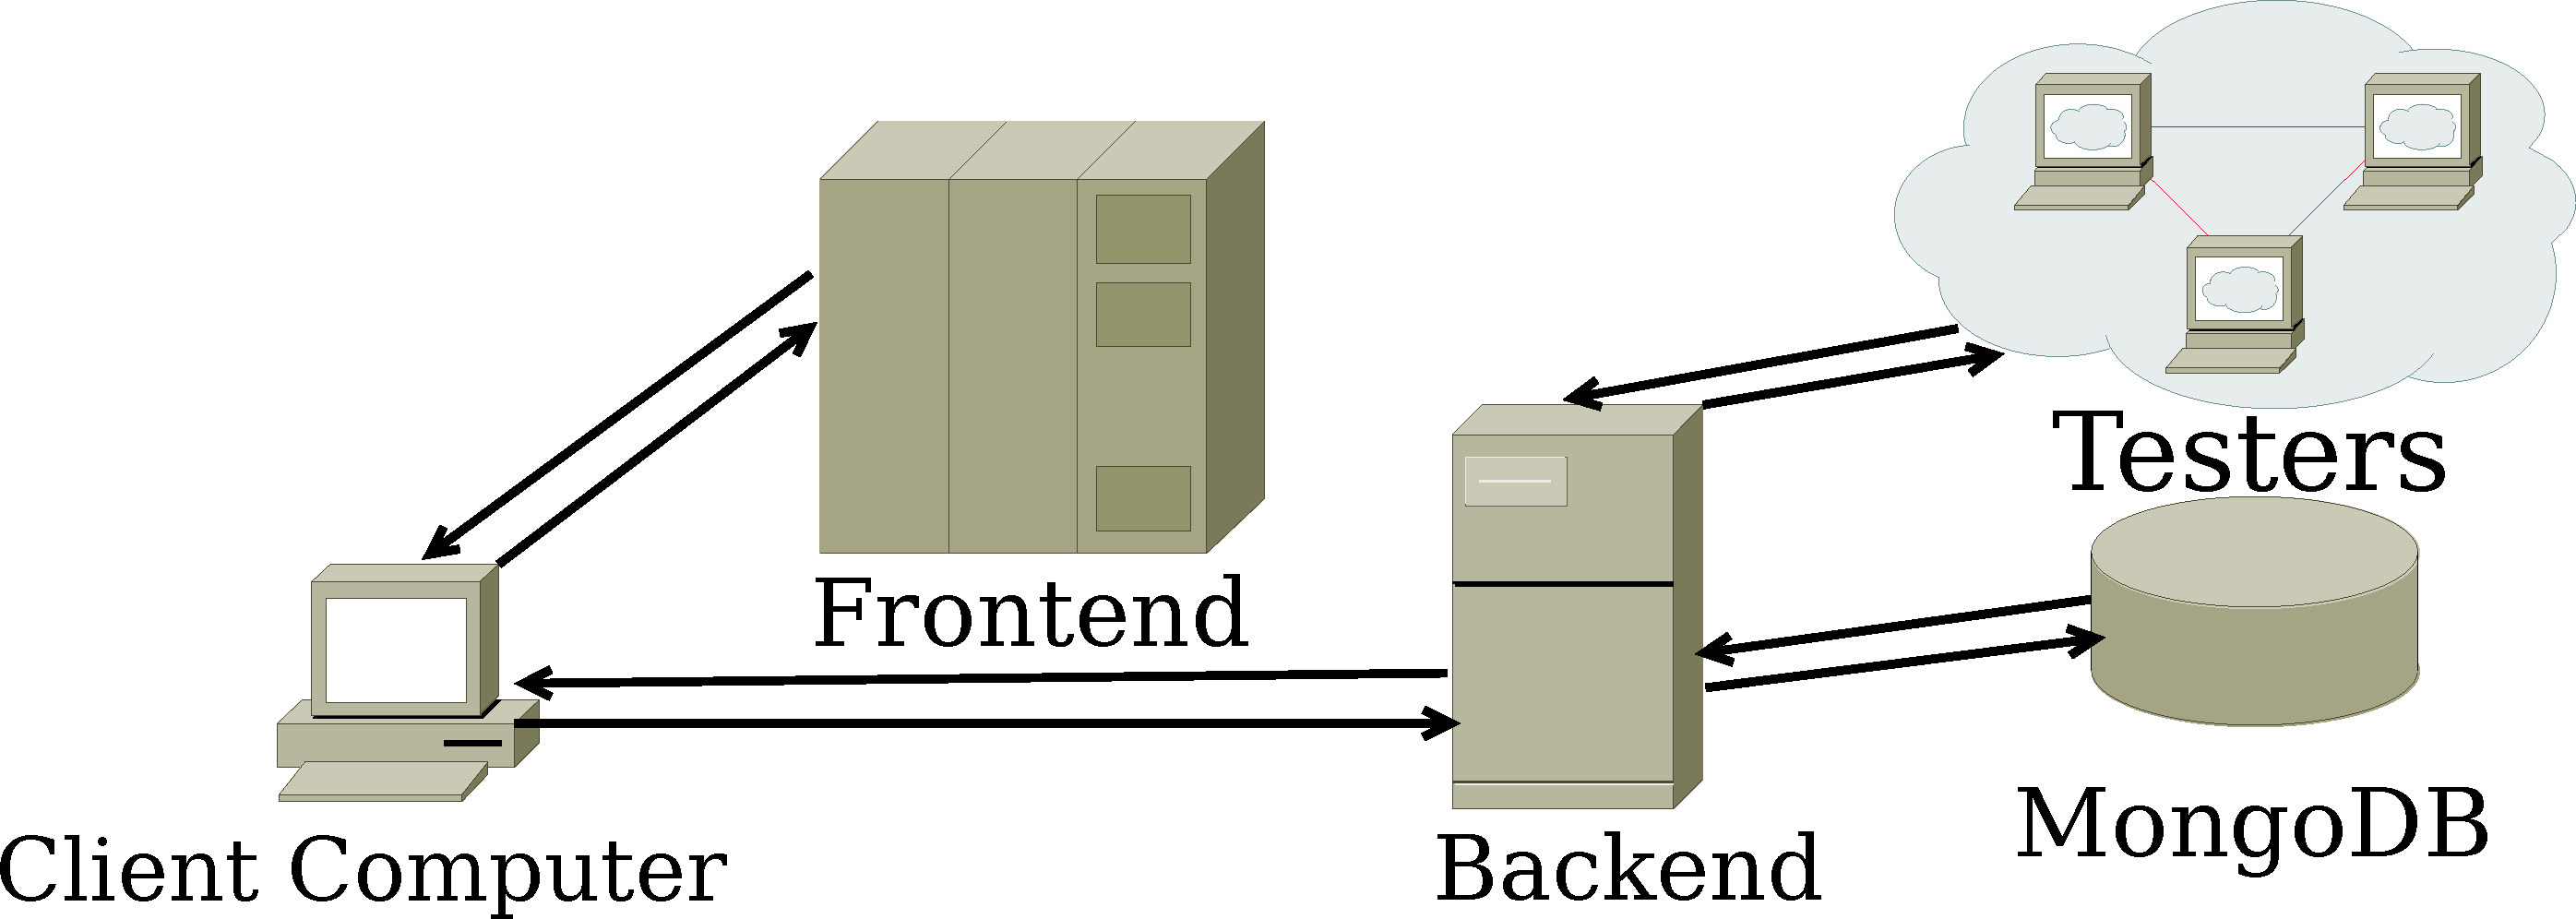
\includegraphics[width=.9\textwidth]{img/architecture.pdf}
\end{figure}

Frontend was designed to avoid keeping state. By doing so, the user-facing components could scale out to multiple backend servers and keep commonly used content cached. This would allow for better load-balancing where frontends could be geographically distributed and yield lower latencies.

Backend was designed to control the database and to keep a centralized management of state transitions. A feature that was discussed, but not investigated, was to shard the data between backends. That would have allowed even greater flexibility in the development of the platform, should it be used in more than one place.

Since tester could be used by other projects than the Gamified Programming Platform, it was designed to be idempotent and stand-alone. This meant that any tester server would yield the same result every time it was queried and have no prior knowledge of the system.


% One could see this as a model-view-controller pattern, where the frontend views the model that is stored in a database and is controlled by the backend. Tester is then used by the backend to analyze code sent from the users.


%In the interviews and the workshop, some features and use cases were identified as candidates for the project see tables~\ref{table:usecase1}--\ref{table:usecase3}. To implement these features, some components such as a website, a utility for testing code and a database were deemed necessary.

%\begin{figure}[hb]
%    \centering
%    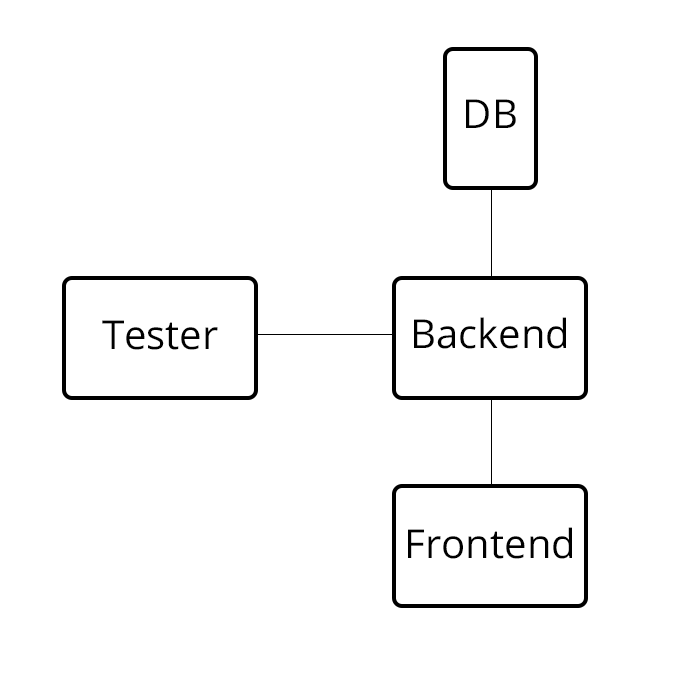
\includegraphics[scale=0.4]{img/SystemA2.png}
%    \caption{A simple sketch over the system parts and how they are connected.}
%\end{figure}

%\begin{table}[H]
\centering
\caption{Use case 1}
\label{my-label}
\begin{tabular}{|l|l|}
\hline
\textbf{Use Case}       & Create Course       
\\ \hline
\textbf{Actor}          & Registered user
\\ \hline
\textbf{Description}    & 
\begin{tabular}[c]{@{}l@{}}
A user logs into the system and opens the page for creating a new\\ course. The user fills in the form and submits the newly created course.
\end{tabular}      
\\ \hline
\textbf{Preconditions}  & \begin{tabular}[c]{@{}l@{}}1. The user is logged into the website\\ 2. The user is either a teacher at LTU or has not \\ created more than three other courses\end{tabular}
\\ \hline
\textbf{Postconditions} & 
\\ \hline
\textbf{Normal flow}    & \begin{tabular}[c]{@{}l@{}}1. The user clicks on the create course button on the user page\\ 2. The user fills in the name and/or the course code \\ 3. The user selects which gamification elements that the \\ course should include \\ 4. The user writes a description for the course\\ 5. The user submits the new course\end{tabular} \\ \hline
\end{tabular}
\end{table}
%\begin{table}[H]
\centering
\caption{Use case 2}
\label{my-label}
\begin{tabular}{|l|l|}
\hline
\textbf{Use Case}       & Submit assignment   
\\ \hline
\textbf{Actor}          & Registered user
\\ \hline
\textbf{Description}    & 
\begin{tabular}[c]{@{}l@{}}
A user logs into the system and enters a course, selects an\\ assignment, writes a solution and then submits the assignment.
\end{tabular}      
\\ \hline
\textbf{Preconditions}  & 
\begin{tabular}[c]{@{}l@{}}
1. The user is logged into the website\\ 
2. The user has joined or created a course with at least one\\ assignment\\ 
\end{tabular}
\\ \hline
\textbf{Postconditions} & 
\begin{tabular}[c]{@{}l@{}}
\textbf{All tests passed}\\
1. The assignment is marked as completed\\
2. Any gamification elements are updated\\ 
\textbf{Assignment failed}\\
1. The user receives feedback of what went wrong\\
\end{tabular}
\\ \hline
\textbf{Normal flow}    & 
\begin{tabular}[c]{@{}l@{}}
1. The user clicks on an assignment inside a course\\ 
2. The user writes a solution to the assignment\\ 
3. The user submits the solution\\ 
\end{tabular} 
\\ \hline
\end{tabular}
\end{table}
%\begin{table}[H]
\centering
\caption{Use case 2}
\label{my-label}
\begin{tabular}{|l|l|}
\hline
\textbf{Use Case}       & Submit assignment   
\\ \hline
\textbf{Actor}          & Registered user
\\ \hline
\textbf{Description}    & 
\begin{tabular}[c]{@{}l@{}}
A user logs into the system and enters a course, selects an\\ assignment, writes a solution and then submits the assignment.
\end{tabular}      
\\ \hline
\textbf{Preconditions}  & 
\begin{tabular}[c]{@{}l@{}}
1. The user is logged into the website\\ 
2. The user has joined or created a course with at least one\\ assignment\\ 
\end{tabular}
\\ \hline
\textbf{Postconditions} & 
\begin{tabular}[c]{@{}l@{}}
\textbf{All tests passed}\\
1. The assignment is marked as completed\\
2. Any gamification elements are updated\\ 
\textbf{Assignment failed}\\
1. The user receives feedback of what went wrong\\
\end{tabular}
\\ \hline
\textbf{Normal flow}    & 
\begin{tabular}[c]{@{}l@{}}
1. The user clicks on an assignment inside a course\\ 
2. The user writes a solution to the assignment\\ 
3. The user submits the solution\\ 
\end{tabular} 
\\ \hline
\end{tabular}
\end{table}

%The system is divided into three parts, frontend, Tester and backend with the database. Tester whose main task is to implement a system that is able to test code that students write and send back the response of the tests. The frontend should visualize the user interface and the gamification parts. The backend is the in the middle and it will forward the code from frontend and load a test from the database, then send the submitted code along with the tests to Tester and then handle the response back to the frontend.

%The decision of what programming language to use was based on the following criteria, it should be fullstack meaning the same language should be used in all the parts for easier collaboration between the software engineers, it should be suitable for web and it should be fairly modern programming language. The two alternatives found was Python with frameworks or JavaScript with frameworks. The chosen programming language was JavaScript using Node.Js for backend and Tester, MongoDB as a NoSQL database and Angular4 for frontend.
